\section{Proposal's context, positioning and objective(s)}
\label{sec:context}

\subsection{Objectives and scientific hypotheses}

\Comments{Present the objectives and the research hypotheses ; present the scientific and technical barriers to be lifted ; present the expected results; if applicable describe any final products developed.}

\noindent\textbf{Context.}
3D volumes come from the segmentation of magnetic resonance, X-ray tomographic or micro-tomographic images. 
They are also generated in scientific modelling and by voxel editors. 
This project is about the geometry of volume boundaries, called \emph{digital surfaces} (fig.~\ref{fig:snow}). 
Keeping the digital nature of the data is an advantage
to use efficient spatial data structures such as voxel octree, 
to perform constructive solid geometry operations,
to do integer-only and exact computations, etc.
A drawback is its poor geometry, because at any resolution a digital surface is only 
made up of quadrangular surface element (\emph{surfel} for short) 
whose normal vector is parallel to one axis. 
Many tasks in computer graphics, vision and 3D image analysis require a richer geometry: 
rendering, surface deformation for simulation or tracking, precise geometric measurements, etc.
To perform relevant geometric tasks and 
to benefit from the above-mentioned advantages in the same time, 
we need to enhance the geometry of digital surfaces by estimating extra data for each surfel. 
This project focuses on estimations of local and first-order geometric quantities: 
normal vector, distance to boundary, coverage of the inner and outer incident voxels 
(see fig.~\ref{fig:2D} for a 2D illustration).  

\begin{figure}[hb]
 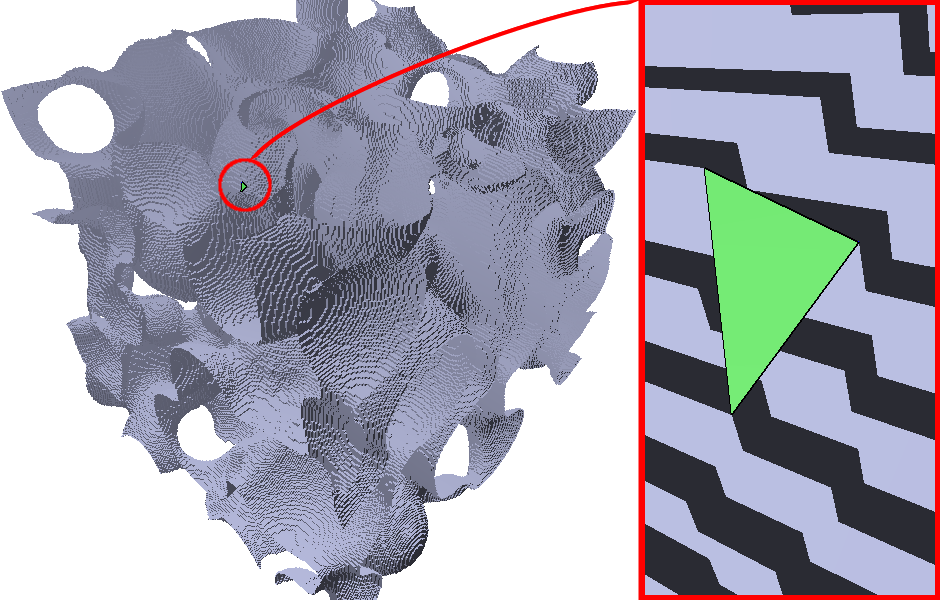
\includegraphics[height=0.2\textheight]{snow-compositionv2.png} %width=0.55\textwidth
 \caption{(a) ``ice-air'' interface in a micro-tomographic image of
   snow\protect\footnotemark~with a closer view to a local normal vector
   estimated by computing a relevant facet.} 
\label{fig:snow} 
\end{figure}
\footnotetext{obtained by the 3SR Lab and CEN/CNRM - GAME URA 1357/M\'{e}t\'{e}o-France - CNRS, 
shared during ANR-11-BS02-009 DigitalSnow project.}

\begin{figure}[hb]
  \centering
\subfloat[]{ 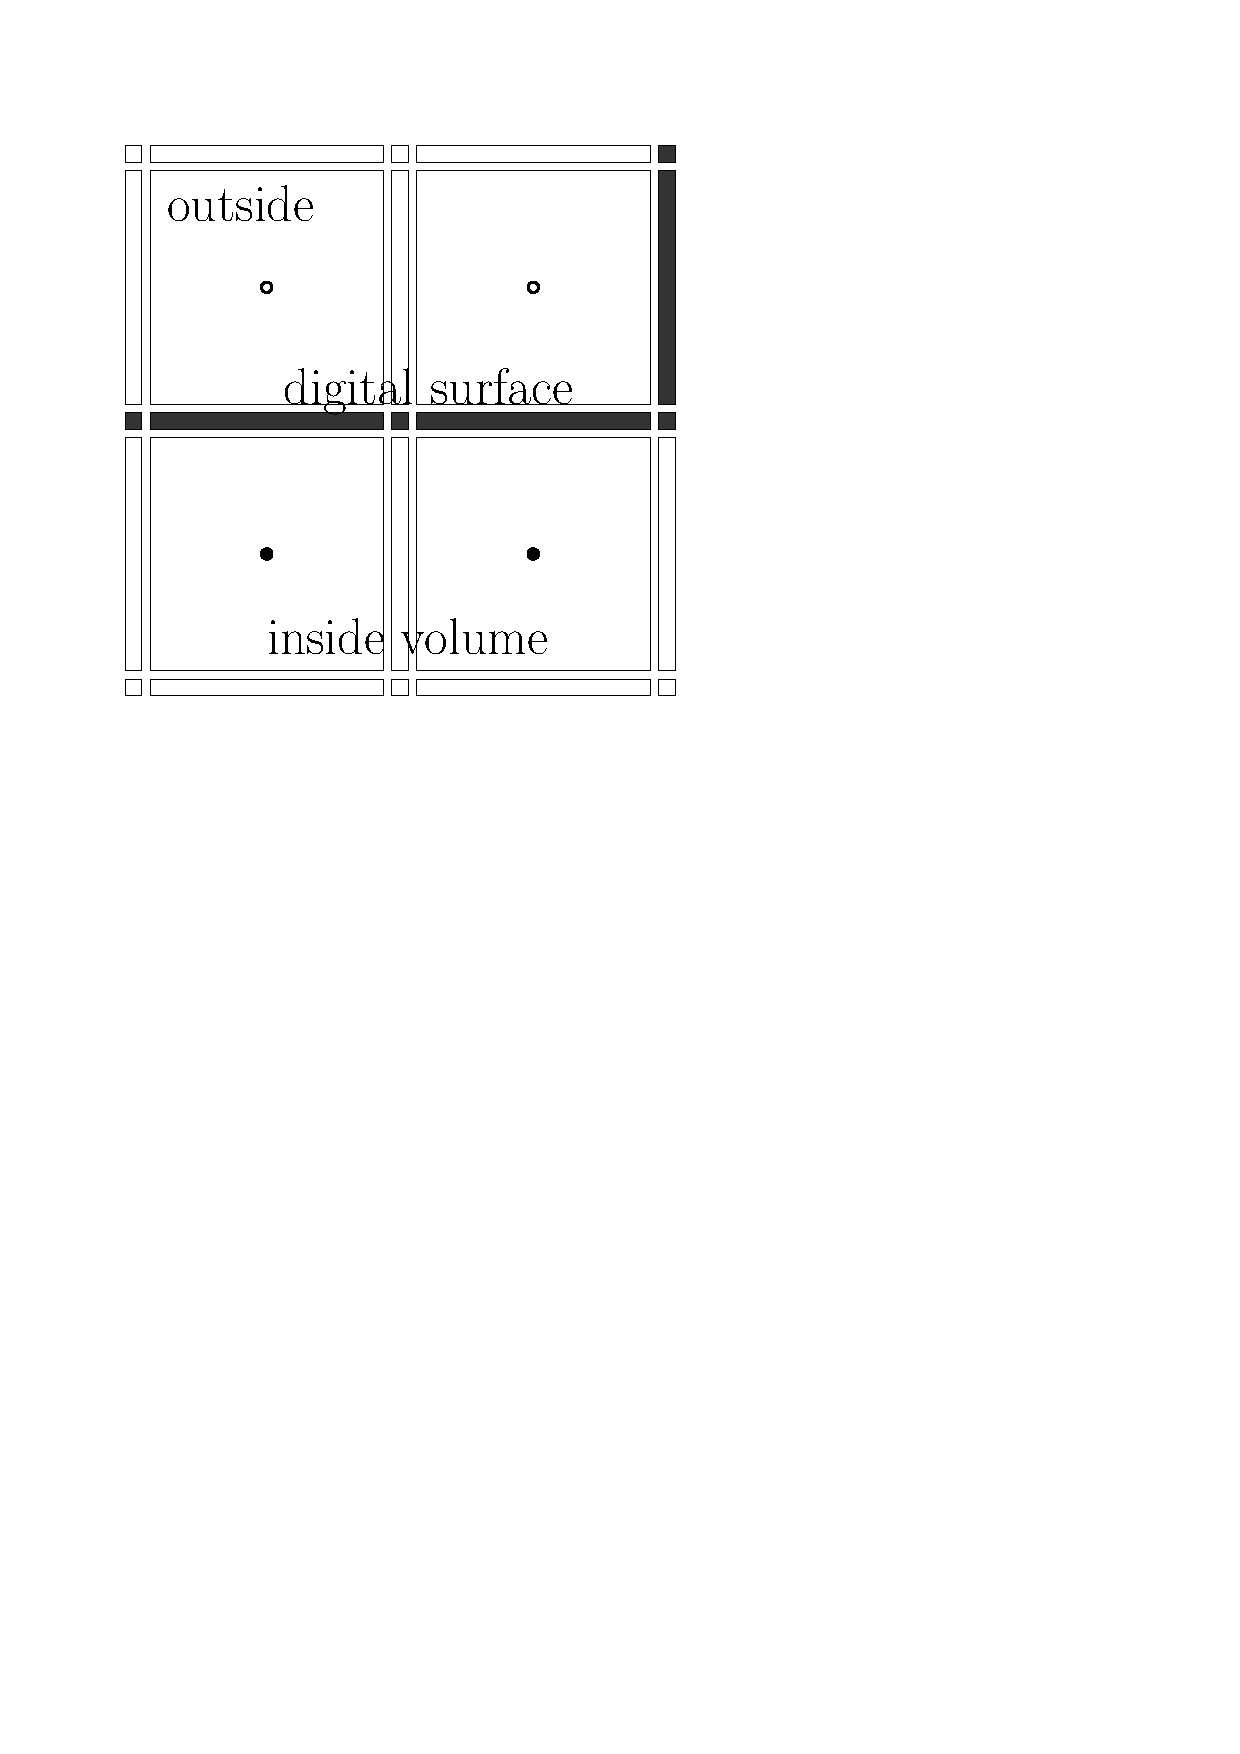
\includegraphics[width=0.17\textwidth,page=1]{square.pdf} } \hspace{0.05\textwidth}
\subfloat[]{ \includegraphics[width=0.17\textwidth,page=2]{square.pdf} } \hspace{0.05\textwidth}
\subfloat[]{ \includegraphics[width=0.17\textwidth,page=3]{square.pdf} } \hspace{0.05\textwidth}
\subfloat[]{ \includegraphics[width=0.17\textwidth,page=4]{square.pdf} } 
 \caption{2D illustration of a digital surface: voxels are big squares whose center is depicted by a black (resp. white) disk if it lies inside (resp. outside) the volume; surfels are elongated dark rectangles. We want to estimate a relevant normal vector at a given surfel (b), but also locally reconstruct a boundary perpendicular to this normal vector in order to derive distance and coverage estimations (c-d).} 
\label{fig:2D} 
\end{figure}

\noindent\textbf{Scientific bottleneck.}
The surface geometry within a patch around each surfel should be gathered to provide such estimations
-- e.g. by polynomial fitting \cite{Cazals2005,Cazals2008}.
Almost all methods require at least one parameter that controls the size of the patch.  
On the other hand, this project aims at providing \emph{accurate} and \emph{parameter-free} estimators
based on a surface patch with \emph{adaptive} size.
%Note that accuracy will be evaluated in a \emph{multigrid-convervence} framework as described in section \ref{sec:wp}, WP2. 
Since we are looking for first-order estimations, the patch will be typically a piece of digital plane
that locally fits to the digital surface. %(fig.~\ref{sub:pattern}).
A challenge is to cover the whole digital surface by maximal pieces of digital plane. 
What makes the problem hard is that there is a combinatorial explosion
of maximal pieces of digital plane \cite{Sivignon2009} and that among them,
not all are tangent to the digital surface in a point set framework.  
An opportunity to make a breakthrough in this issue is the recent development
by the principal investigator and its collaborators of \emph{plane-probing}
algorithms \cite{LPRTCS2016, LPRDGCI2016, LPRJMIV2017}. These algorithms decide
on-the-fly how to probe the digital surface and make grow a piece of digital plane,
which is tangent by construction. The growth direction is given by both arithmetic and geometric properties.

\noindent\textbf{Objectives and expected results.}
The first goal of this project is to study extra arithmetic and combinatorial properties
of plane-probing algorithms. We expect to design an ultimate plane-probing algorithm that
only probes a part of digital surface \emph{as small as possible} to provide a relevant facet.
A formal definition of what is meant by \emph{small} and a theoretical upper bound should be given.
In addition, we expect to be able to make explicit an underlying minimal and connected piece of
digital plane in order to correctly process convex, concave and saddle parts. 

%The algorithm should be implemented in \DGtal at T+12. At the same time, a paper where
%a formal definition of \emph{small} is given with a theoretical upper bound should be ready for
%publication. 
%(see WP0 and WP1 in section~\ref{sec:wp}, describing work packages).

The second goal is to derive \emph{efficient}, \emph{accurate} and \emph{parameter-free} estimators
of \emph{local} and \emph{first-order} geometric quantities: normal vector (and surfel area as a by-product),
distance to boundary, voxel coverage (fig.~\ref{fig:2D}). We expect to derive such estimators from
the above-mentionned plane-probing algorithm and provide a theoretical evaluation of their accuracy
with respect to resolution. Plane-probing algorithms and derived esimators will be implemented in \DGtal.
% at T+24 ?
Theoretical studies and results will be gathered in papers submitted to high impact venues or journals. 
%(WP2).

The third goal is to provide a method and a tool for an automatic and \emph{multiscale} analysis of digital surfaces,
based on the number or the size of the computed facets for several subsampled versions of the input 3D volume. 
We expect to develop a tool that provides, without any parameter, the scale at which noise is unlikely.
This tool will be implemented in \DGtalTools~ and published in \IPOL. 
%(WP3). 

%\todo{expected results and final products}

%1-WP0: algorithm purely local, from any starting point, which leads to a reduced basis and retrieves any normal
%1-WP1: pattern generation: minimal number of tiles, connected, 
%2-WP2: estimateur + ordre de convergence theorique + applis ?
%3-WP3: outils qui prend un volume et sors un sous-échantillon non bruité, ou un ensemble de voxels à différentes tailles (publi IPOL)
%=> for each publication and implementation in DGtal. 

%transition not relevant here
%Since there are so many perspectives and paths to follow, this project needs to strengthen a team of experts by full-time workers in order to make the best of them. 


\subsection{Originality and relevance in relation to the state of the art}

\Comments{Emphasise the ambitious nature of the proposal and the novelty of the research in relation to the state of the art ; show the possible contributions of project partners to the state of the art ; present any preliminary results. In the case of a project proposal following up on previous project(s) already funded by ANR or by another body, provide a summary of the results achieved and clearly describe the new issues raised and the new objectives set out in the light of the earlier project.}

In this section, we review some estimation method in order to underline the novelty of the proposed approach. 

\noindent\textbf{Digital surface and multigrid convergence.}

3D volumes are collections of cubes. % of size $h$, called \emph{grid step}. 
Their topological boundary is a quadrangular mesh called \emph{digital surface}.
The vertex set consists of evenly spaced data points whose coordinates are
half-integer. This set approximates a continuous 2-manifold under a uniform
noise model. 
%TODO: Lachaud Thibert

Most of the time, when we are working with a digital surface, we are 
interested in the geometry of a continuous shape whose digitization
is the input 3D volume.
Formally, given a compact shape $X \subset \R^3$,
its digitization at grid step $h \in \R^+$ is $\Dig(X) := \{z \in \Z^3, hz \in X\}$.
If we denote the axis-aligned closed cube centered on $z \in h\Z^3$ and of size $h$ as $Q_z^h$,
the cube embedding of a digital set $Z$ at grid step $h$ is $\underset{z\in Z}{\cup}Q_z^h$.
Let $\partial_h X$ be the topological boundary of the embedding of the digitization of $X$: 
\[
\partial_h M := \partial \Big( \underset{z\in\Dig(X)}{\bigcup}Q_z^h \Big).
\]

We expect that a given geometric quantity, such as a normal vector,
computed at a point of a digital surface ($\partial_h X$),
is close to the one of the underlying continuous shape ($X$) at a close enough point. 

\begin{Definition}[multigrid-convergent estimator \cite{Coeurjolly2012}]
  \label{def:multigrid-convergence2}
  The estimator $\hat{Q}$ is {\em multigrid-convergent} for the family
  {\Shapes} if and only if, for any shape $X \in \Shapes$,
  there exists a grid step $h_X>0$ such that the estimate
    $\hat{Q}(\Dig(X),y,h)$ is defined for all
  $y \in \partial_h X$ with $0<h < h_X$, and for any $x \in \BT{X}$,
  \begin{equation*}
    \forall y \in \partial_h X \text{~with~} \| y - x \|_1 \le h, \quad
    \hat{Q}(\Dig(X),y,h) - Q(X,x) | \le \tau_{X,x}(h),
  \end{equation*}
  where $\tau_{X,x}: \R^{+*} \rightarrow \R^+$ has null limit at
  $0$.
  %% This function defines the speed of convergence of $\hat{Q}$
  %% toward $Q$ at point $x$ of $\BT{X}$. The convergence is {\em uniform} for
  %% $X$ when every $\tau_{X,x}$ is bounded from above by a function
  %% $\tau_X$ independent of $x \in \BT{X}$ with null limit at $0$.
\end{Definition}

The accuracy of a multigrid-convergent estimator depends on the grid step:
the smaller the grid step, the more accurate the estimator. 


%TODO: dire pourquoi c'est interessant de regarder ce qui se fait en point cloud, quel lien avec les digital surfaces
%ou alors presenter les donnees et la convergence multigrille

%TODO: pourquoi c'est interessant des normales ?

%TODO
% Je parlerais des methodes 2d convergentes dans multigrid convergence
%Provot and Gérard show the multigrid convergence of an estimator based on a
%polynomial fitting for digitization of TODO \cite{Provot2011}.
%\cite{Provot2011,Esbelin2011,Esbelin2016}

\noindent\textbf{Normal estimation in 3d.}

Hoppe \etal estimate the normal at a given data point by computing
the least squares best fitting plane to a point set within a neighborhood
around the point of interest \cite{Hoppe1992}.
Other fitting surfaces have been used too, such as jets, \ie truncated Taylor expansion
of a surface expression \cite{Cazals2005,Cazals2008}. 

All fitting methods first consist in collecting the points used for the fitting.
In the mesh case, a breadth-first search visit the neighbors until enough points
have been collected. In the point-cloud case, we typically resort to the k-nearest-neighbors
strategy. In both cases, the number of points to collect is usually a user-defined parameter,
even if some heuristics are proposed to select it automatically \cite{Hoppe1992,Cazals2005}.  

%In 3d, a straightforward application
%of \cite{Cazals2005}[Theorem 3] to digital surface shows that a polynomial fitting of degree $n$
%estimates the coefficients of the unit normal vector in $O(h^n)$.
%TRIS probablement faux

Instead of approximating the tangent space, another familly of methods focuses on the
Voronoi diagram to estimate at best the orthogonal space. Amenta \etal first use the
furthest vertex of the Voronoi cell to estimate the normals of point clouds \cite{Amenta1999}.
In order to get more stable estimates, Alliez \etal propose to apply linear fitting
to the Voronoi cell or to the union of Voronoi cells into a neighborhood \cite{Alliez2007}. 
Mérigot \etal propose an improvement, called Voronoi Covariance Measure (VCM),
by taking a weighted average of covariance matrices of Voronoi cells instead of
taking the covariance matrix of their union \cite{Merigot2011}. In their method,
only the intersection between the Voronoi diagram and a ball around the data point
are taken into account in order to get purely local information about the surface geometry.
A digital variant has been proposed by Cuel \etal \cite{Cuel2015}. 

In the mesh case, another method sums up the surface geometry within a ball by 
computing integrals over the intersection between the ball and the volume
bounded by the mesh \cite{Pottmann2009}. The covariance matrix of the intersection set 
provides a way to estimate principal curvatures, principal directions and normal direction.
A digital variant has been proposed by Lachaud \etal \cite{Lachaud2017}.

The radius of the ball is a user-defined parameter in these methods. The above-mentionned
digital variants \cite{Cuel2015,Lachaud2017} are multigrid convergent for digitization
of smooth shapes if the radius is conveniently chosen with respect to the grid step.

\todo{by convolution}
%pas d'isotropie, donc filtres
%bilateral mesh denoising
%\cite{Fourey2009}

To end, let us mention also probabilistic methods based on the Randomized Hough Transform.
Boulch and Marlet consider many random triples of data points in a neighborhood
and bin their normal direction into a spherical histogram \cite{Boulch2012}.
Maximal vote provides the normal estimate. However, their method has many input parameters,
the first of which is the size or radius of the neighborhood. 

\noindent\textbf{Parameter-free estimators.}

2d \cite{Lachaud2007}

3d  

To the best of our knowledge, on digital surfaces, only one parameter-free normal estimator
has been proposed in nD (see \cite{Lachaud2003} and references therein for 3D).
It is based on maximal digital straight segments on 2D slices.
Maximal digital straight segments provide windows of adaptive size
but the slicing truncates the geometric information and leads to
an artificial spatial variability because two neighbor surfels only
share one slice over two.

%methods using DSS size for 
%David: II ?
%Tris: pour l'estimation de normale, c'est un peu over-kill, mais c'est juste, plus généralement pour toute les méthodes qui ont un parametre de taille (même si la convergence n'est pas prouvée). En parler dans la proposition...

 %=> plan discret / explosion combinatoire / pas d'ordre
\noindent\textbf{Recognition of digital plane segment.}
Related works usually make grow a point set by a breadth-first search according to some heuristics and decide whether the current set is a piece of digital plane or not \cite{Sivignon2004,Charrier2011}. The results are highly dependent on the chosen heuristics.   
%TODO citation de David sur la reconnaissance de plans discrets ?
% => breadth-first search + heuristics pour grandir

%thomas fernique en lien avec la section suivante. 

\noindent\textbf{Digital plane generation.}
%substitution methode generale


\noindent\textbf{Preliminary results.}
%lister les avantages, les limites ?

\subsection{c. Methodology and risk management}

\Comments{Describe the methods and technical decisions, risks and fall-back solutions envisaged.}

%methodes: 
%plane-probing algorithms sont une bonne approche pour etre tangent, local, sans parametre,
%substitution bonne approche pour generer un motif au cours de l'algorithme
%lien avec env. conv. bonne approche pour preuve estimateur et analyse multi-echelle

%risques:
%algos pas parfaits: il en existe actuellement un 
%\Comments{Le risque est réduit par les travaux exploratoires des participants au projet.}
%motif genere pas bons:
 %- on les genere apres coup en faisant une sorte de croissance de regions
 %- on traite les concavites avec un critere de separation
%l'estimateur n'est pas convergent: peu probable, mais si ça arrive c'est que les motifs sont trop petits, il ne grandisse pas assez vite par rapport au pas h, dans ce cas on agrandit le motif jusqu'à obtenir m surfels, ou on agrandit jusqu'à avoir une épaisseur <= h, ou on combine des motifs voisins.


\subsection{pre-proposition}

%version 2, pour avoir une entree en matiere plus grand public. 
\noindent\textbf{Context.} 
3D volumes come from the segmentation of magnetic resonance, X-ray tomographic or micro-tomographic images. 
They are also generated in scientific modelling and by voxel editors. 
This project is about the geometry of volume boundaries, called \emph{digital surfaces} (fig.~\ref{sub:snow}). 
Keeping the digital nature of the data is an advantage
to use efficient spatial data structures such as voxel octree, 
to perform constructive solid geometry operations,
to do integer-only and exact computations, etc.
A drawback is its poor geometry, because at any resolution a digital surface is only 
made up of quadrangular surface element (\emph{surfel} for short) 
whose normal vector is parallel to one axis. 
Many tasks in computer graphics, vision and 3D image analysis require a richer geometry: 
rendering, surface deformation for simulation or tracking, precise geometric measurements, etc.
To perform relevant geometric tasks and 
to benefit from the above-mentioned advantages in the same time, 
we need to enhance the geometry of digital surfaces by estimating extra data for each surfel. 
This project focuses on estimations of local and first-order geometric quantities: 
normal vector, distance to boundary, coverage of the inner and outer incident voxels 
(see fig.~\ref{sub:2D} for a 2D illustration).  


\begin{figure}[hb]
 \subfloat[]{ 
 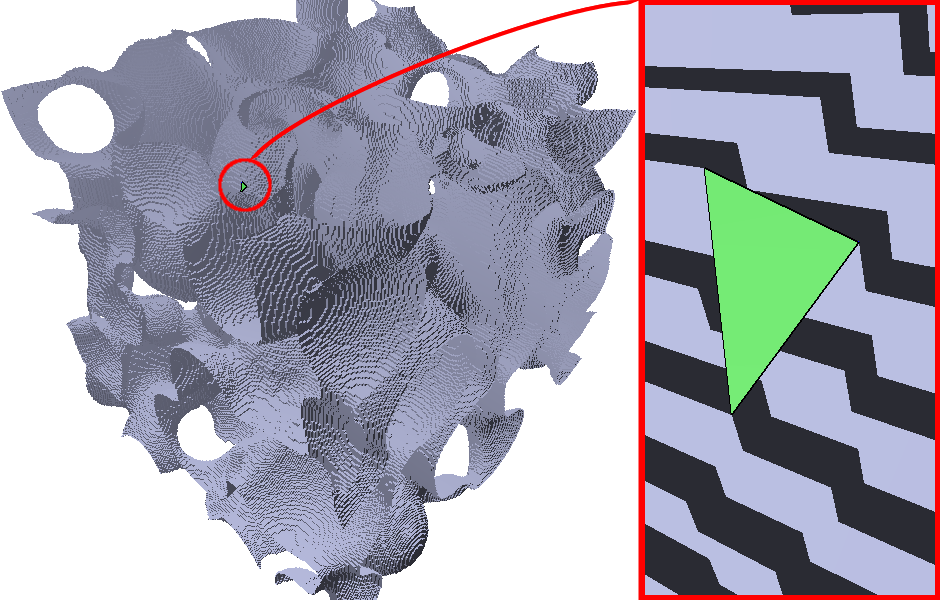
\includegraphics[height=0.2\textheight]{snow-compositionv2.png} %width=0.55\textwidth
 \label{sub:snow}
 }
% \subfloat[]{
%  \includegraphics[width=0.25\textwidth,angle=90,origin=b,trim=40 40 10 60,clip=true]{onPlane2-6-11.eps} %
% \label{sub:pattern}
% }
 \subfloat[]{
  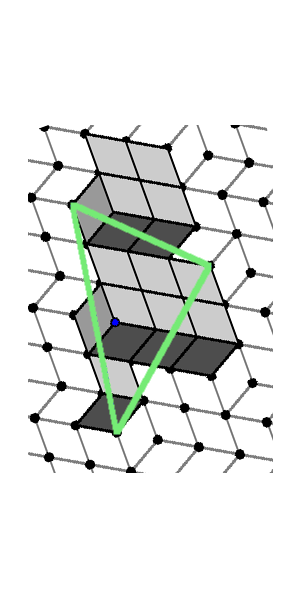
\includegraphics[height=0.2\textheight]{pattern-green.png} %
 \label{sub:pattern}
 }
 \subfloat[]{
\begin{tabular}[b]{cc}
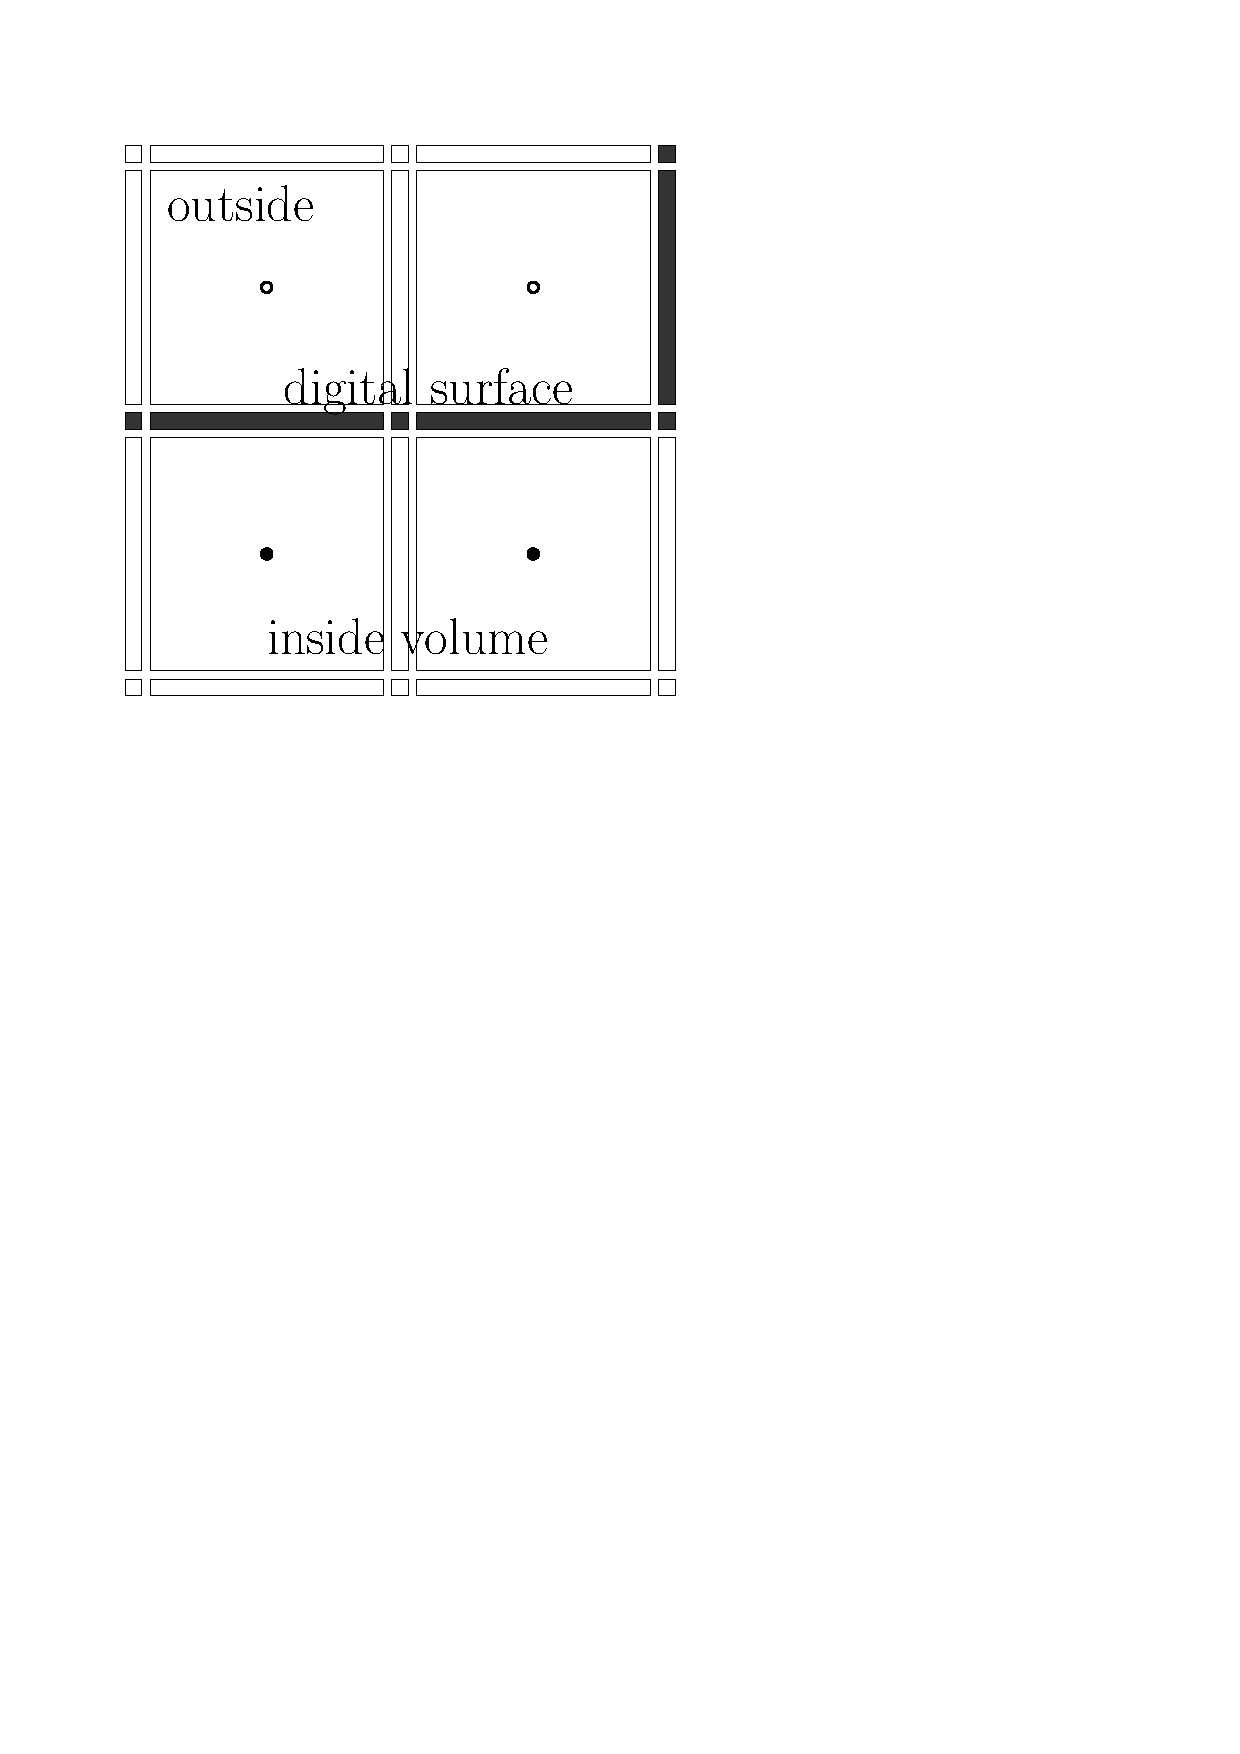
\includegraphics[width=0.145\textwidth,page=1]{square.pdf} &
\includegraphics[width=0.145\textwidth,page=2]{square.pdf} \\
\includegraphics[width=0.145\textwidth,page=3]{square.pdf} &
\includegraphics[width=0.145\textwidth,page=4]{square.pdf} \\
\end{tabular}
 \label{sub:2D}
 }
% \subfloat[]{ 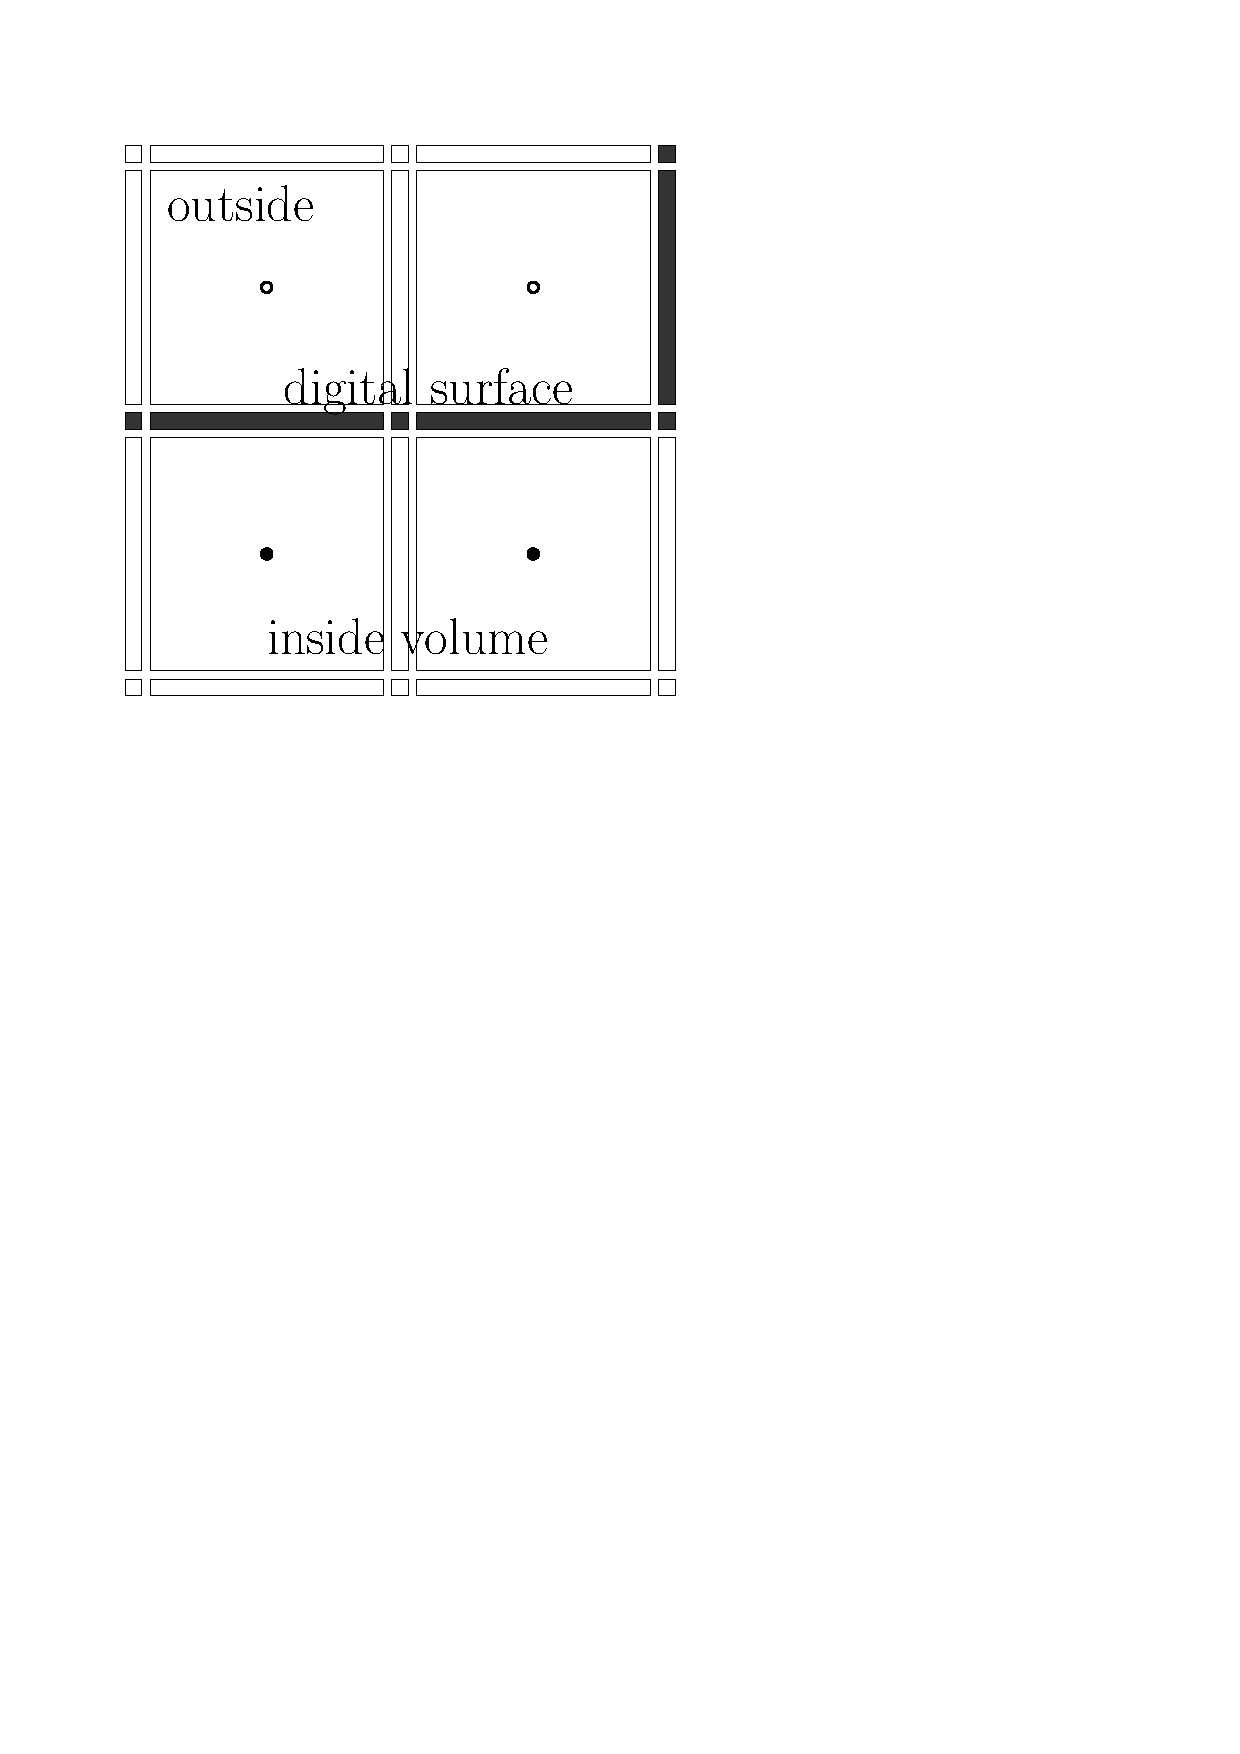
\includegraphics[width=0.17\textwidth,page=1]{square.pdf} } \hspace{0.05\textwidth}
% \subfloat[]{ \includegraphics[width=0.17\textwidth,page=2]{square.pdf} } \hspace{0.05\textwidth}
% \subfloat[]{ \includegraphics[width=0.17\textwidth,page=3]{square.pdf} } \hspace{0.05\textwidth}
% \subfloat[]{ \includegraphics[width=0.17\textwidth,page=4]{square.pdf} } 
 \caption{(a) ``ice-air'' interface in a micro-tomographic image of snow\protect\footnotemark~with a closer view to a local normal vector estimated by computing a relevant facet. (b) Piece of digital plane that locally fits to the surface. (c) 2D illustration of a digital surface: voxels are big squares whose center is depicted by a black (resp. white) disk if it lies inside (resp. outside) the volume; surfels are elongated dark rectangles. We want to estimate a relevant normal vector at a given surfel (top right), but also locally reconstruct a boundary perpendicular to this normal vector in order to derive distance and coverage estimations (bottom row).} 
\label{fig:ex} 
\end{figure}
 %\dav{(former ANR Project digitalSnow)}.
\footnotetext{obtained by the 3SR Lab and CEN/CNRM - GAME URA 1357/M\'{e}t\'{e}o-France - CNRS, 
shared during ANR-11-BS02-009 DigitalSnow project.}

\noindent\textbf{Positioning and scientific bottleneck.}
The surface geometry within a patch around each surfel should be gathered to provide such estimations -- e.g. by convolution \cite{Pottmann2009} or polynomial fitting \cite{Cazals2008}.
Almost all methods require at least one parameter that controls the size of the patch.  

To the best of our knowledge, on digital surfaces, only one parameter-free normal estimator has been proposed in nD (see \cite{Lachaud2003} and references therein for 3D). It is based on maximal digital straight segments on 2D slices. Maximal digital straight segments provide windows of adaptive size but the slicing truncates the geometric information and leads to an artificial spatial variability because two neighbor surfels only share one slice over two.     
%David: II ?
%Tris: pour l'estimation de normale, c'est un peu over-kill, mais c'est juste, plus généralement pour toute les méthodes qui ont un parametre de taille (même si la convergence n'est pas prouvée). En parler dans la proposition...

Is it possible to provide \emph{accurate} and \emph{parameter-free} estimators based on a surface patch with \emph{adaptive} size?
%Note that accuracy will be evaluated in a \emph{multigrid-convervence} framework as described in section \ref{sec:wp}, WP2. 
Since we are looking for first-order estimations, the patch will be typically a piece of digital plane that locally fits to the digital surface (fig.~\ref{sub:pattern}). A challenge is to cover the whole digital surface by maximal pieces of digital plane. 
What makes the problem hard is that there is a combinatorial explosion of maximal pieces of digital plane \cite{Sivignon2009} and that among them, not all are tangent to the digital surface in a point set framework.  
Related works usually make grow a point set by a breadth-first search according to some heuristics and decide whether the current set is a piece of digital plane or not \cite{Sivignon2004,Charrier2011}. The results are highly dependent on the chosen heuristics.   
%TODO citation de David sur la reconnaissance de plans discrets ?

\noindent\textbf{Objectives.}
An opportunity to make a breakthrough in this issue is the recent development by the principal investigator and its collaborators of \emph{plane-probing} algorithms \cite{LPRTCS2016, LPRDGCI2016, LPRJMIV2017}. These algorithms decide on-the-fly how to probe the digital surface and make grow a piece of digital plane, which is tangent by construction. The growth direction is given by both arithmetic and geometric properties.

The first goal of this project is to study extra arithmetic and combinatorial properties of plane-probing algorithms (see WP0 and WP1 in section~\ref{sec:wp}, describing work packages). The second one is to derive \emph{efficient}, \emph{accurate} and \emph{parameter-free} estimators of \emph{local} and \emph{first-order} geometric quantities (WP2). The third one is to provide a method and a tool for an automatic and \emph{multiscale} analysis of digital surfaces (WP3). 
Since there are so many perspectives and paths to follow, this project needs to strengthen a team of experts by full-time workers in order to make the best of them. 
%a person working full-time in a team of experts in order to make the best of them. 
